% This template was originally by R. Jacob Vogelstein
% Updated on March 1, 2010 by Noah J. Cowan
% Updated on January 29, 2016 by John Muschelli
% Updated on April 13, 2016 by Leonardo Collado Torres

\documentclass[12pt]{report}

%% This was the setup recommended at https://github.com/weitzner/jhu-thesis-template
% \documentclass[12pt,oneside,final]{thesis}

\pdfminorversion=5
\pdfobjcompresslevel=0
\usepackage[a-1b]{pdfx} % Need this to create a PDF/A file

\usepackage{pdfpages}

\pagestyle{myheadings}
%\topmargin=0.25in
\topmargin=0.05in
\textheight=8.15in
\textwidth=5.6in
\oddsidemargin=0.7in
\raggedbottom
\newdimen \jot \jot=5mm
\brokenpenalty=10000
 

%\usepackage[utf8]{inputenc} % Seems to cause a conflict with fontenc and lmodern
%\DeclareUnicodeCharacter{00A0}{ }
\usepackage[T1]{fontenc}
\usepackage{lmodern} % load a font with all the characters
%\usepackage{hyperref}
\usepackage{tocbibind} % need this to contents adding for TOC
\usepackage{setspace}
\setstretch{1.05}
\usepackage{RJournal_nogeom} % Changes the colors of links among other things
%\usepackage[all]{hypcap}
\usepackage[hypcap=true]{caption}
\hypersetup{linktocpage}
\usepackage{amsmath,amssymb,array}
\usepackage{booktabs}
\usepackage{subfig}

%% load any required packages here
\usepackage{graphicx}
\usepackage{float}
\usepackage{tikz}
\usepackage{graphics} 
\usetikzlibrary{positioning}
\usetikzlibrary{shapes,arrows}
\usepackage{dcolumn}
% A math shortcut frequently used by John Muschelli
\newcommand{\bbeta}{\mbox{\boldmath $\beta$}}

%%%%%%%%%%%%%%%%%%%%%%%%%%%%%%%%%%%%%%%%%%%%%%%%%%%%%%%%%%%%%%%%
% DOI from Segmentation
% Don't use - needs hyperref
%%%%%%%%%%%%%%%%%%%%%%%%%%%%%%%%%%%%%%%%%%%%%%%%%%%%%%%%%%%%%%%%
%\makeatletter
%\providecommand{\doi}[1]{%
%  \begingroup
%    \let\bibinfo\@secondoftwo
%    \urlstyle{rm}%
%    \href{http://dx.doi.org/#1}{%
%      doi:\discretionary{}{}{}%
%      \nolinkurl{#1}%
%    }%
%  \endgroup
%}
%\makeatother

%%%%%%%%%%%%%%%%%%%%%%%%%%%%%%%%%%%%%%%%%%%%%%%%%%%%%%%%%%%%%%%%
% StartKNITR STUFF -- added by John Muschelli
%%%%%%%%%%%%%%%%%%%%%%%%%%%%%%%%%%%%%%%%%%%%%%%%%%%%%%%%%%%%%%%%
\usepackage{color}
%% maxwidth is the original width if it is less than linewidth
%% otherwise use linewidth (to make sure the graphics do not exceed the margin)
\makeatletter
\def\maxwidth{ %
  \ifdim\Gin@nat@width>\linewidth
    \linewidth
  \else
    \Gin@nat@width
  \fi
}
\makeatother

\definecolor{fgcolor}{rgb}{0.345, 0.345, 0.345}
\newcommand{\hlnum}[1]{\textcolor[rgb]{0.686,0.059,0.569}{#1}}%
\newcommand{\hlstr}[1]{\textcolor[rgb]{0.192,0.494,0.8}{#1}}%
\newcommand{\hlcom}[1]{\textcolor[rgb]{0.678,0.584,0.686}{\textit{#1}}}%
\newcommand{\hlopt}[1]{\textcolor[rgb]{0,0,0}{#1}}%
\newcommand{\hlstd}[1]{\textcolor[rgb]{0.345,0.345,0.345}{#1}}%
\newcommand{\hlkwa}[1]{\textcolor[rgb]{0.161,0.373,0.58}{\textbf{#1}}}%
\newcommand{\hlkwb}[1]{\textcolor[rgb]{0.69,0.353,0.396}{#1}}%l
\newcommand{\hlkwc}[1]{\textcolor[rgb]{0.333,0.667,0.333}{#1}}%
\newcommand{\hlkwd}[1]{\textcolor[rgb]{0.737,0.353,0.396}{\textbf{#1}}}%

\usepackage{framed}
\makeatletter
\newenvironment{kframe}{%
 \def\at@end@of@kframe{}%
 \ifinner\ifhmode%
  \def\at@end@of@kframe{\end{minipage}}%
  \begin{minipage}{\columnwidth}%
 \fi\fi%
 \def\FrameCommand##1{\hskip\@totalleftmargin \hskip-\fboxsep
 \colorbox{shadecolor}{##1}\hskip-\fboxsep
     % There is no \\@totalrightmargin, so:
     \hskip-\linewidth \hskip-\@totalleftmargin \hskip\columnwidth}%
 \MakeFramed {\advance\hsize-\width
   \@totalleftmargin\z@ \linewidth\hsize
   \@setminipage}}%
 {\par\unskip\endMakeFramed%
 \at@end@of@kframe}
\makeatother

\definecolor{shadecolor}{rgb}{.97, .97, .97}
\definecolor{messagecolor}{rgb}{0, 0, 0}
\definecolor{warningcolor}{rgb}{1, 0, 1}
\definecolor{errorcolor}{rgb}{1, 0, 0}
\newenvironment{knitrout}{}{} % an empty environment to be redefined in TeX
\makeatletter
\newcommand\gobblepars{%
    \@ifnextchar\par%
        {\expandafter\gobblepars\@gobble}%
        {}}
\makeatother
%%%%%%%%%%%%%%%%%%%%%%%%%%%%%%%%%%%%%%%%%%%%%%%%%%%%%%%%%%%%%%%%
% End KNITR STUFF
%%%%%%%%%%%%%%%%%%%%%%%%%%%%%%%%%%%%%%%%%%%%%%%%%%%%%%%%%%%%%%%%


\usepackage[
style = authoryear, 
sorting = none, 
dashed = false,
maxbibnames = 99,
backend = bibtex,
natbib = true
]{biblatex}

% If you want to exclude some portions from the bibliography
\AtEveryBibitem{
\clearfield{note}
\clearfield{month}
}


\usepackage{enumerate}

%\tolerance=10000

%\makeglossary % enable the glossary
\graphicspath{{rnw_chapter/figure/}{rnw_chapter/}} % change it accordingly!


\setcounter{tocdepth}{4}
\setcounter{secnumdepth}{4}
\begin{document}

\newcommand{\bm}[1]{ \mbox{\boldmath $ #1 $} }
\newcommand{\bin}[2]{\left(\begin{array}{@{}c@{}} #1 \\ #2
             \end{array}\right) }
\renewcommand{\contentsname}{Table of Contents}
\baselineskip=24pt
 
% Create cover page of dissertation !
\pagenumbering{roman}
\thispagestyle{empty}
\begin{center}
\vspace*{.25in}
{\bf\LARGE{ JHU Thesis Template title }}\\ % change it accordingly!
\vspace*{.75in}
{\bf by} \\*[18pt]
\vspace*{.2in}
{\bf Your Name}\\ % change it accordingly!
\vspace*{1in}
{\bf A dissertation submitted to The Johns Hopkins University\\
in conformity with the requirements for the degree of\\
Doctor of Philosophy }\\
\vspace*{.75in}
{\bf Baltimore, Maryland} \\
{\bf June, 2016} \\     % change it accordingly!
\vspace*{.5in}
\begin{small}
{\bf \copyright{ }2016 by Your Name} \\ % change the year if needed!
{\bf All rights reserved}
\end{small}
\end{center}
\newpage 

% Add acknowledgements
\chapter*{Abstract}

My thesis is about bla bla

\chapter*{Thesis Committee}

\section*{}
\subsection*{Primary Readers}

\begin{singlespace}


\indent First Lastname (Primary Advisor)\\
\indent \indent Assistant Professor \\
\indent \indent Department of ChangeMe\\
\indent \indent  Johns Hopkins Bloomberg School of Public Health \\


\smallskip 

\noindent First Lastname \\
\indent \indent Assistant Professor\\
\indent \indent Department of ChangeMe\\
\indent \indent  Johns Hopkins Bloomberg School of Public Health \\

\smallskip 

\noindent First Lastname \\
\indent \indent Assistant Professor\\
\indent \indent Department of ChangeMe \\
\indent \indent Johns Hopkins Bloomberg School of Public Health \\

\smallskip


\noindent First Lastname \\
\indent \indent Associate Professor\\
\indent \indent Affiliation1, and\\
\indent \indent Department1 \& Department2 at\\
\indent \indent Johns Hopkins Bloomberg School of Public Health \\


\end{singlespace}

\subsection*{Alternate Readers}

\begin{singlespace}


\indent First Lastname  \\
\indent \indent Professor\\
\indent \indent Department of ChangeMe\\
\indent \indent  Johns Hopkins Bloomberg School of Public Health \\

\noindent First Lastname  \\
\indent \indent Assistant Professor\\
\indent \indent Department of ChangeMe\\
\indent \indent  Johns Hopkins Bloomberg School of Public Health \\




\end{singlespace}
















\chapter*{Acknowledgments}

Thanks!

%\cleardoublepage
%\newpage 
\pagestyle{plain}
\baselineskip=24pt
\tableofcontents
% for the three lines below, change the page numbers if needed!
%\addtocontents{toc}{\contentsline{chapter}{Table of Contents}{iii}}
%\addtocontents{toc}{\protect\contentsline{chapter}{\protect\numberline{}Table of Contents}{iii}}
%\addtocontents{toc}{\protect\contentsline{chapter}{\protect\numberline{}List of Tables}{iv}}
%\addtocontents{toc}{\protect\contentsline{chapter}{\protect\numberline{}List of Figures}{v}}
\listoftables
\listoffigures

\cleardoublepage % Needed because our intro chapter doesn't really have anything
\pagenumbering{arabic}


% add your chapters, best way is to have separate TeX files for each chapter
%%% FRONTMATTER
\begin{frontmatter}

% generate title
\maketitle

\begin{abstract}

Abstract goes here.

\vspace{1cm}

\noindent Primary Reader: Some Person\\
Secondary Reader: Someone Else

\end{abstract}

\begin{acknowledgment}

Thanks!

\end{acknowledgment}

\begin{dedication}
 
This thesis is dedicated to \ldots

\end{dedication}

% generate table of contents
\tableofcontents

% generate list of tables
\listoftables

% generate list of figures
\listoffigures

\end{frontmatter}

%\chapter{Introduction}
\label{sec:intro}
\chaptermark{Optional running chapter heading}

Introduction.

A citation \cite{A}. 
A citation without brackets \citen{B}. 
Multiple citations \cite{A, B, C}.

\section{Section}
\label{sec:section}

This is a section.  Here's a reference to a different section:
\ref{sec:subsection}.

\subsection{Subsection}
\label{sec:subsection}

This is a subsection.

% \begin{figure}[t]
% \centering
% \includegraphics[width=\textwidth]{figure}
% \makeatletter
% \let\@currsize\normalsize
% \caption{Caption.}
% \label{fig:figure}
% \end{figure}
% 
% \begin{figure}[t]
% \centering
% \begin{tabular}{c c}
% \includegraphics[height=2.5in]{figureA} &
% \includegraphics[width=3in]{figureB}\\
% (A) & (B)
% \end{tabular}
% \makeatletter
% \let\@currsize\normalsize
% \caption{Two figures.}
% \label{fig:twofigures}
% \end{figure}

% currsize is not set in the long table environment, so we need to set it before we set it up.
\makeatletter
\let\@currsize\normalsize
\makeatother

% tabular environments are set to be single-spaced in the  thesis class,  but long tables do not use tabular
% to get around this, set the spacing to single spacing at the start of the long table environment, and set it back to double-spacing at the end of it
\ssp
\begin{longtable}{cc}
\caption[This is what I want to have in the LOT]{This is a caption.} \label{tab:pfams} \\
\hline
A & B \\
\hline
\endfirsthead
\multicolumn{2}{@{}l}{\textbf{Table \thetable} \ldots continued} \\
\hline
A & B \\
\hline
\endhead
a1 & b1 \\
a2 & b2 \\
a3 & b3 \\
a4 & b4 \\
\hline
\end{longtable}
\dsp

\section[Optional table of contents heading]{Section with\\linebreaks in\\the
name}

This is another section.

\subsection{Another subsection}

\subsubsection{Subsubsection}

\paragraph{Heading level below subsubsection}
\label{sec:paragraph}

And I quote: 
%
\begin{quote}
La la la.
\end{quote}
%
\noindent No ident after end of quote.  

Another paragraph with a list:
%
\begin{itemize}
%  
\item Item 1
%
\item Item 2
%
\end{itemize}
%
\noindent Again, we don't indent here.

%% The above was the recommended setup by https://github.com/weitzner/jhu-thesis-template but it's no longer needed
%% after Muschelli's changes which stores different chapters in their
%% respective directories. You will still need to add your chapters as
%% TeX files or Rnw files (see rnw_chapter as an example) and please
%% remember to update the makefile accordingly.

\begin{refsection}[intro_chapter/intro_chapter.bib]
\chapter{Introduction}
\label{chap:intro}

Introduce your thesis

\cleardoublepage
\printbibliography[title={References}]
\end{refsection}

\begin{refsection}[rnw_chapter/rnw_chapter.bib]
\chapter{Rnw example chapter}
\label{chap:rnw}





This document was generated on Wed Apr 13 18:01:10 2016.

As shown in Figure \ref{fig:some_fig} and in Table \ref{tab:rtab1} we can see that bla bla \citep{B}.


\begin{knitrout}
\definecolor{shadecolor}{rgb}{0.969, 0.969, 0.969}\color{fgcolor}\begin{figure}
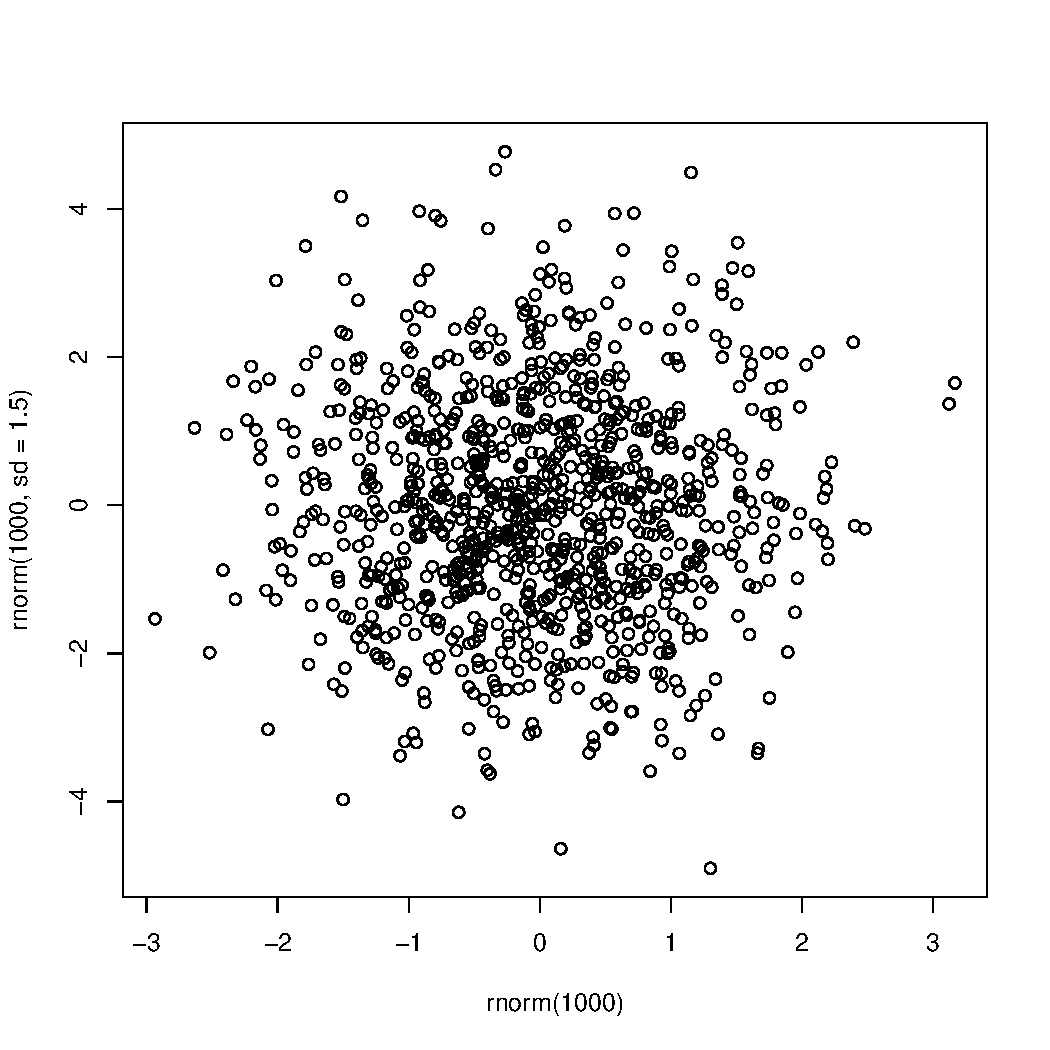
\includegraphics[width=\maxwidth]{figure/some_fig-1} \caption[{\bf Figure title } Rest of description]{{\bf Figure title } Rest of description}\label{fig:some_fig}
\end{figure}


\end{knitrout}






% latex table generated in R 3.3.0 by xtable 1.8-2 package
% Wed Apr 13 18:01:10 2016
\begin{table}[ht]
\centering
\begin{tabular}{rr}
  \hline
A & B \\ 
  \hline
  1 & -0.40 \\ 
    2 & -1.27 \\ 
    3 & -1.04 \\ 
    4 & 0.69 \\ 
    5 & 0.08 \\ 
    6 & 1.71 \\ 
    7 & 1.90 \\ 
    8 & 1.88 \\ 
    9 & 0.17 \\ 
   10 & -1.62 \\ 
   \hline
\end{tabular}
\caption{\bf{ Table title } Table description} 
\label{tab:rtab1}
\end{table}


\cleardoublepage
\printbibliography[title={References}]
\end{refsection}

\begin{refsection}[conclusion_chapter/conclusion_chapter.bib]
\chapter{Discussion and Conclusion}
\label{chap:conclusion}

Discuss and conclude your thesis

\cleardoublepage
\printbibliography[title={References}]
\end{refsection}


% CV PDF file downloaded from the moderncv template available at Overleaf
% https://www.overleaf.com/latex/templates/modern-cv-and-cover-letter-2015-version/sttkgjcysttn#.Vw6PFRMrL65
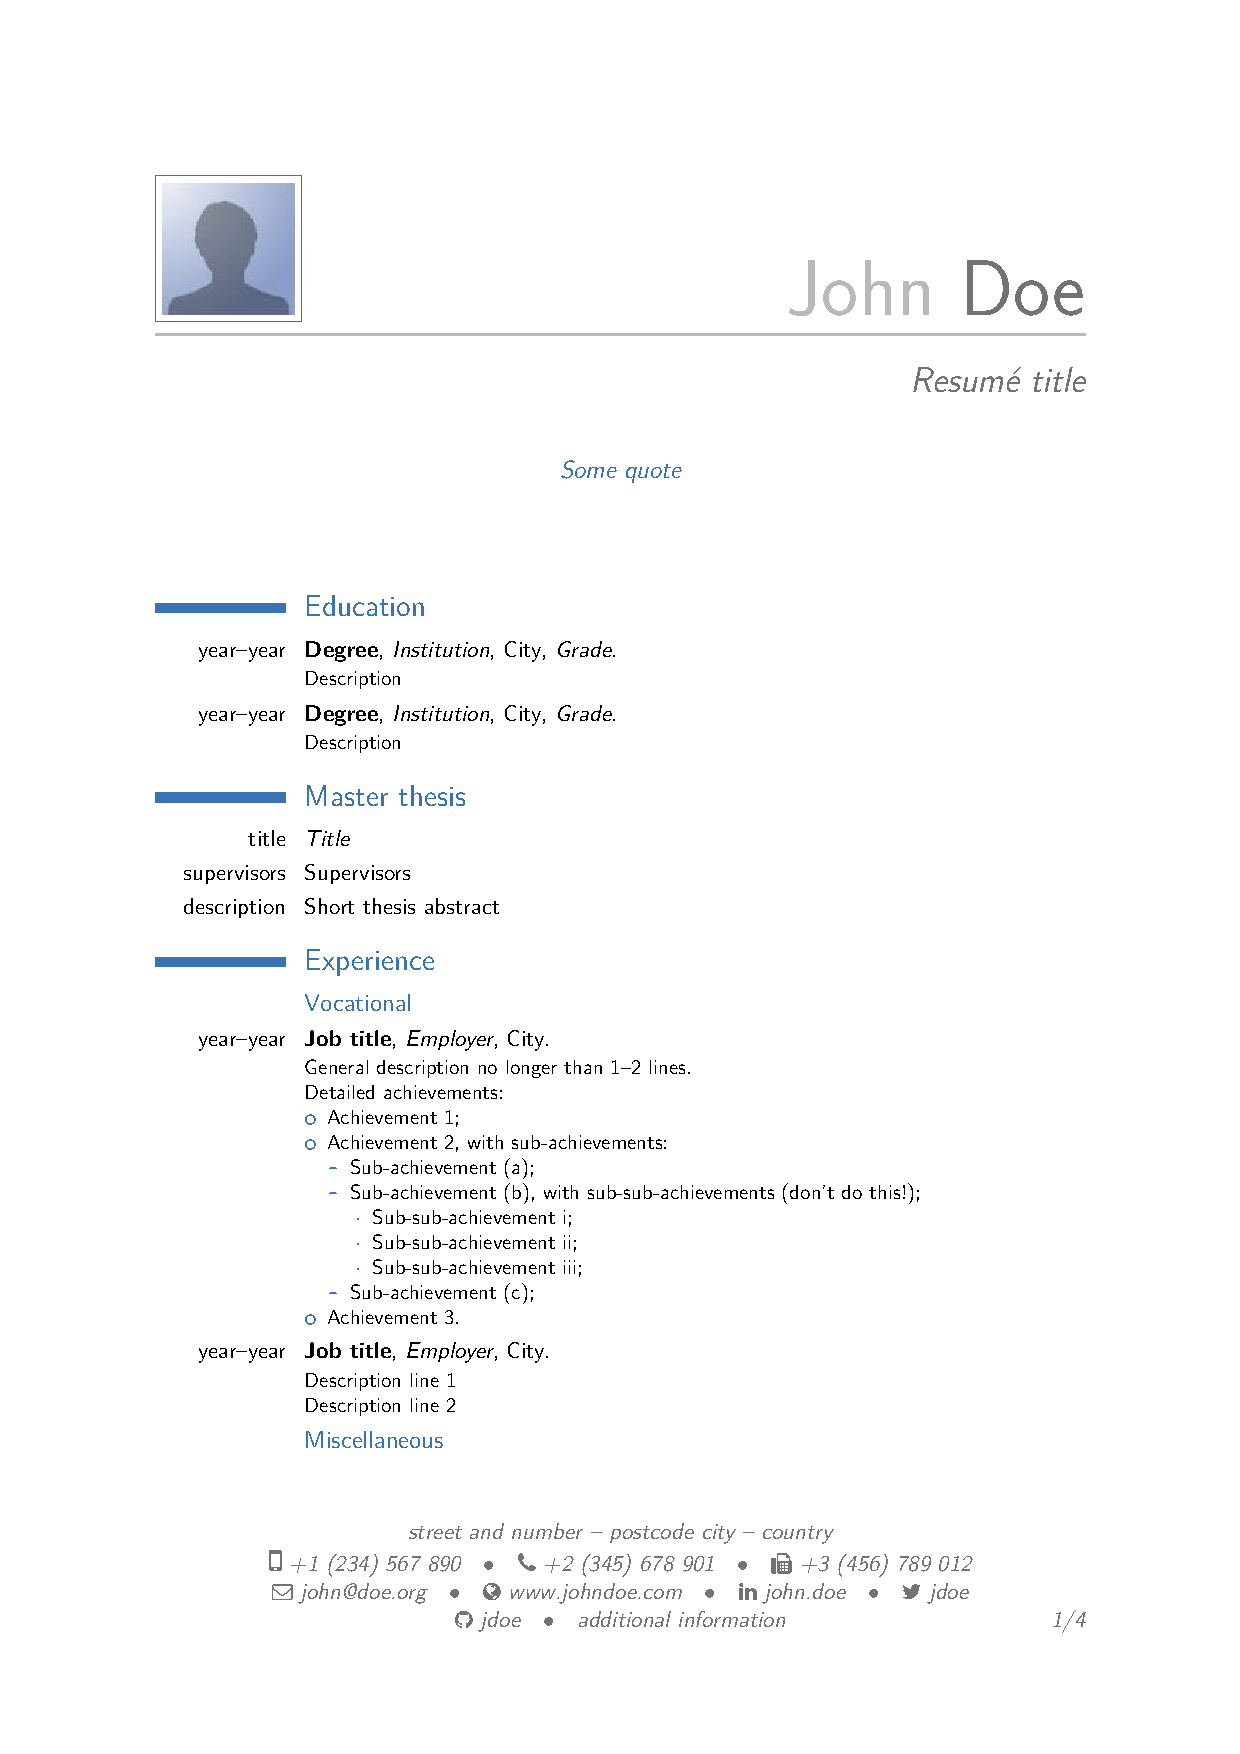
\includepdf[pages={-}]{moderncv-2015.pdf}


\end{document}
